\documentclass{scrartcl}
\usepackage[letterpaper, top=1.5cm, left=1.5cm, right=1.5cm, bottom=2.5cm]{geometry}
\usepackage{hyperref}
\usepackage{graphicx}
\usepackage{csquotes}

\setcounter{secnumdepth}{0} % Remove numbering from sections
\setlength{\parindent}{0cm} % Remove indent from new paragraph
\setlength{\parskip}{6pt} % Add line of whitespace after paragraph
\graphicspath{ {figs/} }

\begin{document}
\title{\vspace{-1cm}\textbf{OSF Meetings Guide}}
\subtitle{Preparing for EEID 2023}
\maketitle

\vspace*{-1cm}

\tableofcontents

\section{\underline{Submitting Your Poster/Talk}}

This year, EEID is using the Open Science Framework (OSF) as a way for presenters to upload their presentations ahead of the conference, allowing attendees to view them before, during, and after the conference.
This not only benefits attendees, but also presenters, as it gives the opportunity for viewers to think critically about your work allowing for more detailed and in-depth discussions during the conference.
While it is not a requirement to upload your presentation, we strongly encourage you to do as a means to enhance the conference experience for everyone.


To submit your poster, or talk, you should first create an account on the OSF website (\href{https://osf.io/}{\texttt{https://osf.io/}}) if you do not already have one.

\subsection{Creating an OSF Account}

If you navigate to the OSF website, you will see a button in the top right corner labelled \texttt{Sign Up}.
Clicking on this will take you to a page where you can create an account.
The are a number of options available to you, but we would strongly suggest that you sign up directly with your email address.
If you have an ORCiD account, you should sign up with the same email address as your ORCiD account, as this will make it easier to link your ORCiD account to your OSF account.


\begin{displayquote}
    \textbf{Note:} While you can sign up for OSF with your ORCiD account, we do not recommend this method as occasionally the email address associated with your ORCiD account does not get transferred correctly to OSF.
    Notably, it sometimes excludes periods in your email address, so when you submit your poster or talk, it will be as if you submitted from a different email address, and you will not be able to edit your submission.
\end{displayquote}

Once you sign up, you will receive an email from OSF asking you to verify your email address.

\subsection{Linking Your ORCiD Account}

To link your ORCiD account to your OSF account, the only thing you need to do is log out of OSF, then \emph{Sign In}, but this time click on the \emph{Sign in with ORCiD} button.
Enter your full name and email address as they appear in OSF (this should be the same as your ORCiD account), press \emph{Submit}, and then click on the verification link you will be emailed.

\subsection{Emailing Your Poster/Talk}

Once you have created an OSF account, you just need to email your poster/talk to EEID. Please ensure your email comes from the email address you used to create your OSF account/linked through ORCiD.

\begin{itemize}
    \item To submit a poster, send an email to: \href{mailto:EEID2023-poster@osf.io}{\texttt{EEID2023-poster@osf.io}}
    \item To submit a talk, send an email to: \href{mailto:EEID2023-talk@osf.io}{\texttt{EEID2023-talk@osf.io}}
\end{itemize}

The email should contain three components, as shown in Figure \ref{fig:submission-email}:

\begin{enumerate}
    \item \textbf{Email subject}: The title of your poster/talk.
    If you do not title your email, your poster/talk will not be added to OSF.
    \item \textbf{Message body}: The abstract of your poster/talk.
    This will be copied verbatim (without formatting) to the \emph{Wiki} of the OSF project that will be set up, so please do not include any extra text in the body of the email.
    Like markdown or \LaTeX, to create line breaks in your abstract, you will need to leave a blank line between paragraphs, i.e., 

    \begin{verbatim}
        This is the first line.
        
        This is the second line.
    \end{verbatim}

    not

    \begin{verbatim}
        This is the first line.
        This is the second line.
    \end{verbatim}

    \item \textbf{Attachment}: The poster/talk file.
    Talk files can be in any format.
    In-person posters need to be 36 inches x 46 inches (in either landscape or portrait orientation).
    Posters that will not be presented in-person can be any size, but should attempt to stay close to the 36 inches x 46 inches size.

\end{enumerate}

\begin{figure}[!htb]
    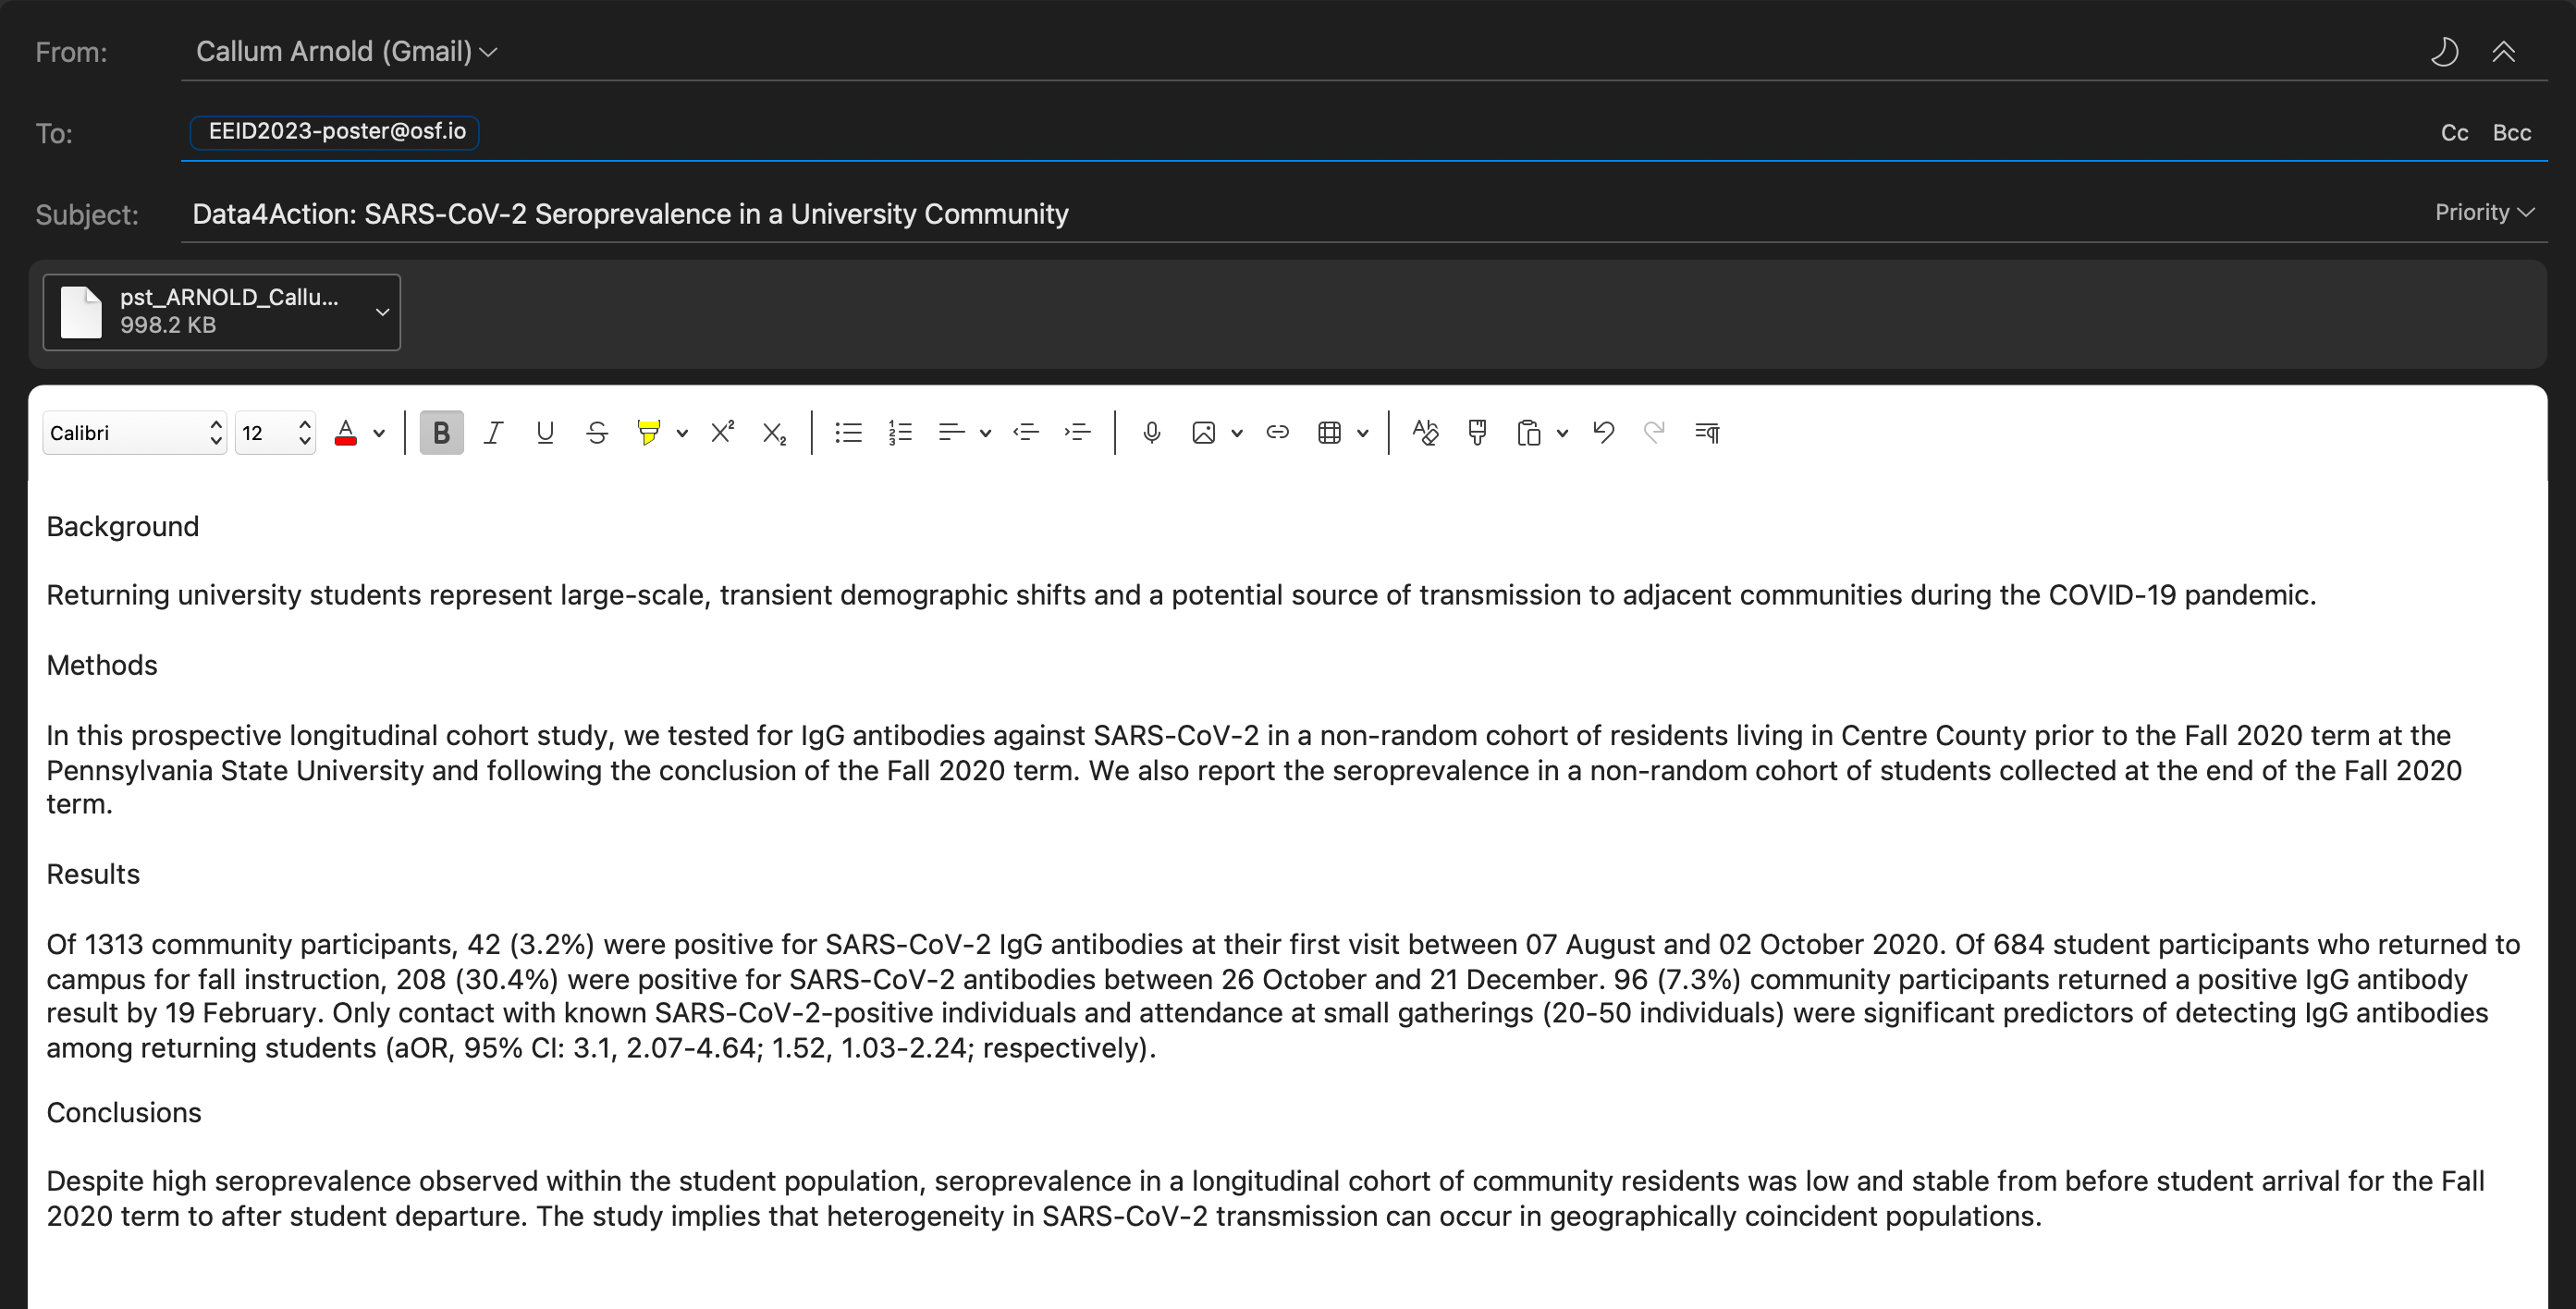
\includegraphics[width=\textwidth]{submission-email.png}
    \caption{Submission Email}
    \label{fig:submission-email}
\end{figure}



Upon receiving your email, we will create an OSF project (in your OSF account) for your poster/talk, and upload the file you sent us.
This project will be linked to the EEID 2023 conference page, and will be publicly viewable, but only editable by you.

\section{\underline{Viewing Posters/Talks}}

Upon submission of your poster/talk, you will receive an email from OSF with two links: the first is a permanent citable URL for your poster/talk project, and the second is a link to the EEID 2023 conference page.

Clicking on the first link (to your project), you will see a page like the one below (you will need to log in to OSF account if you are not already logged in).

\begin{figure}[!htb]
    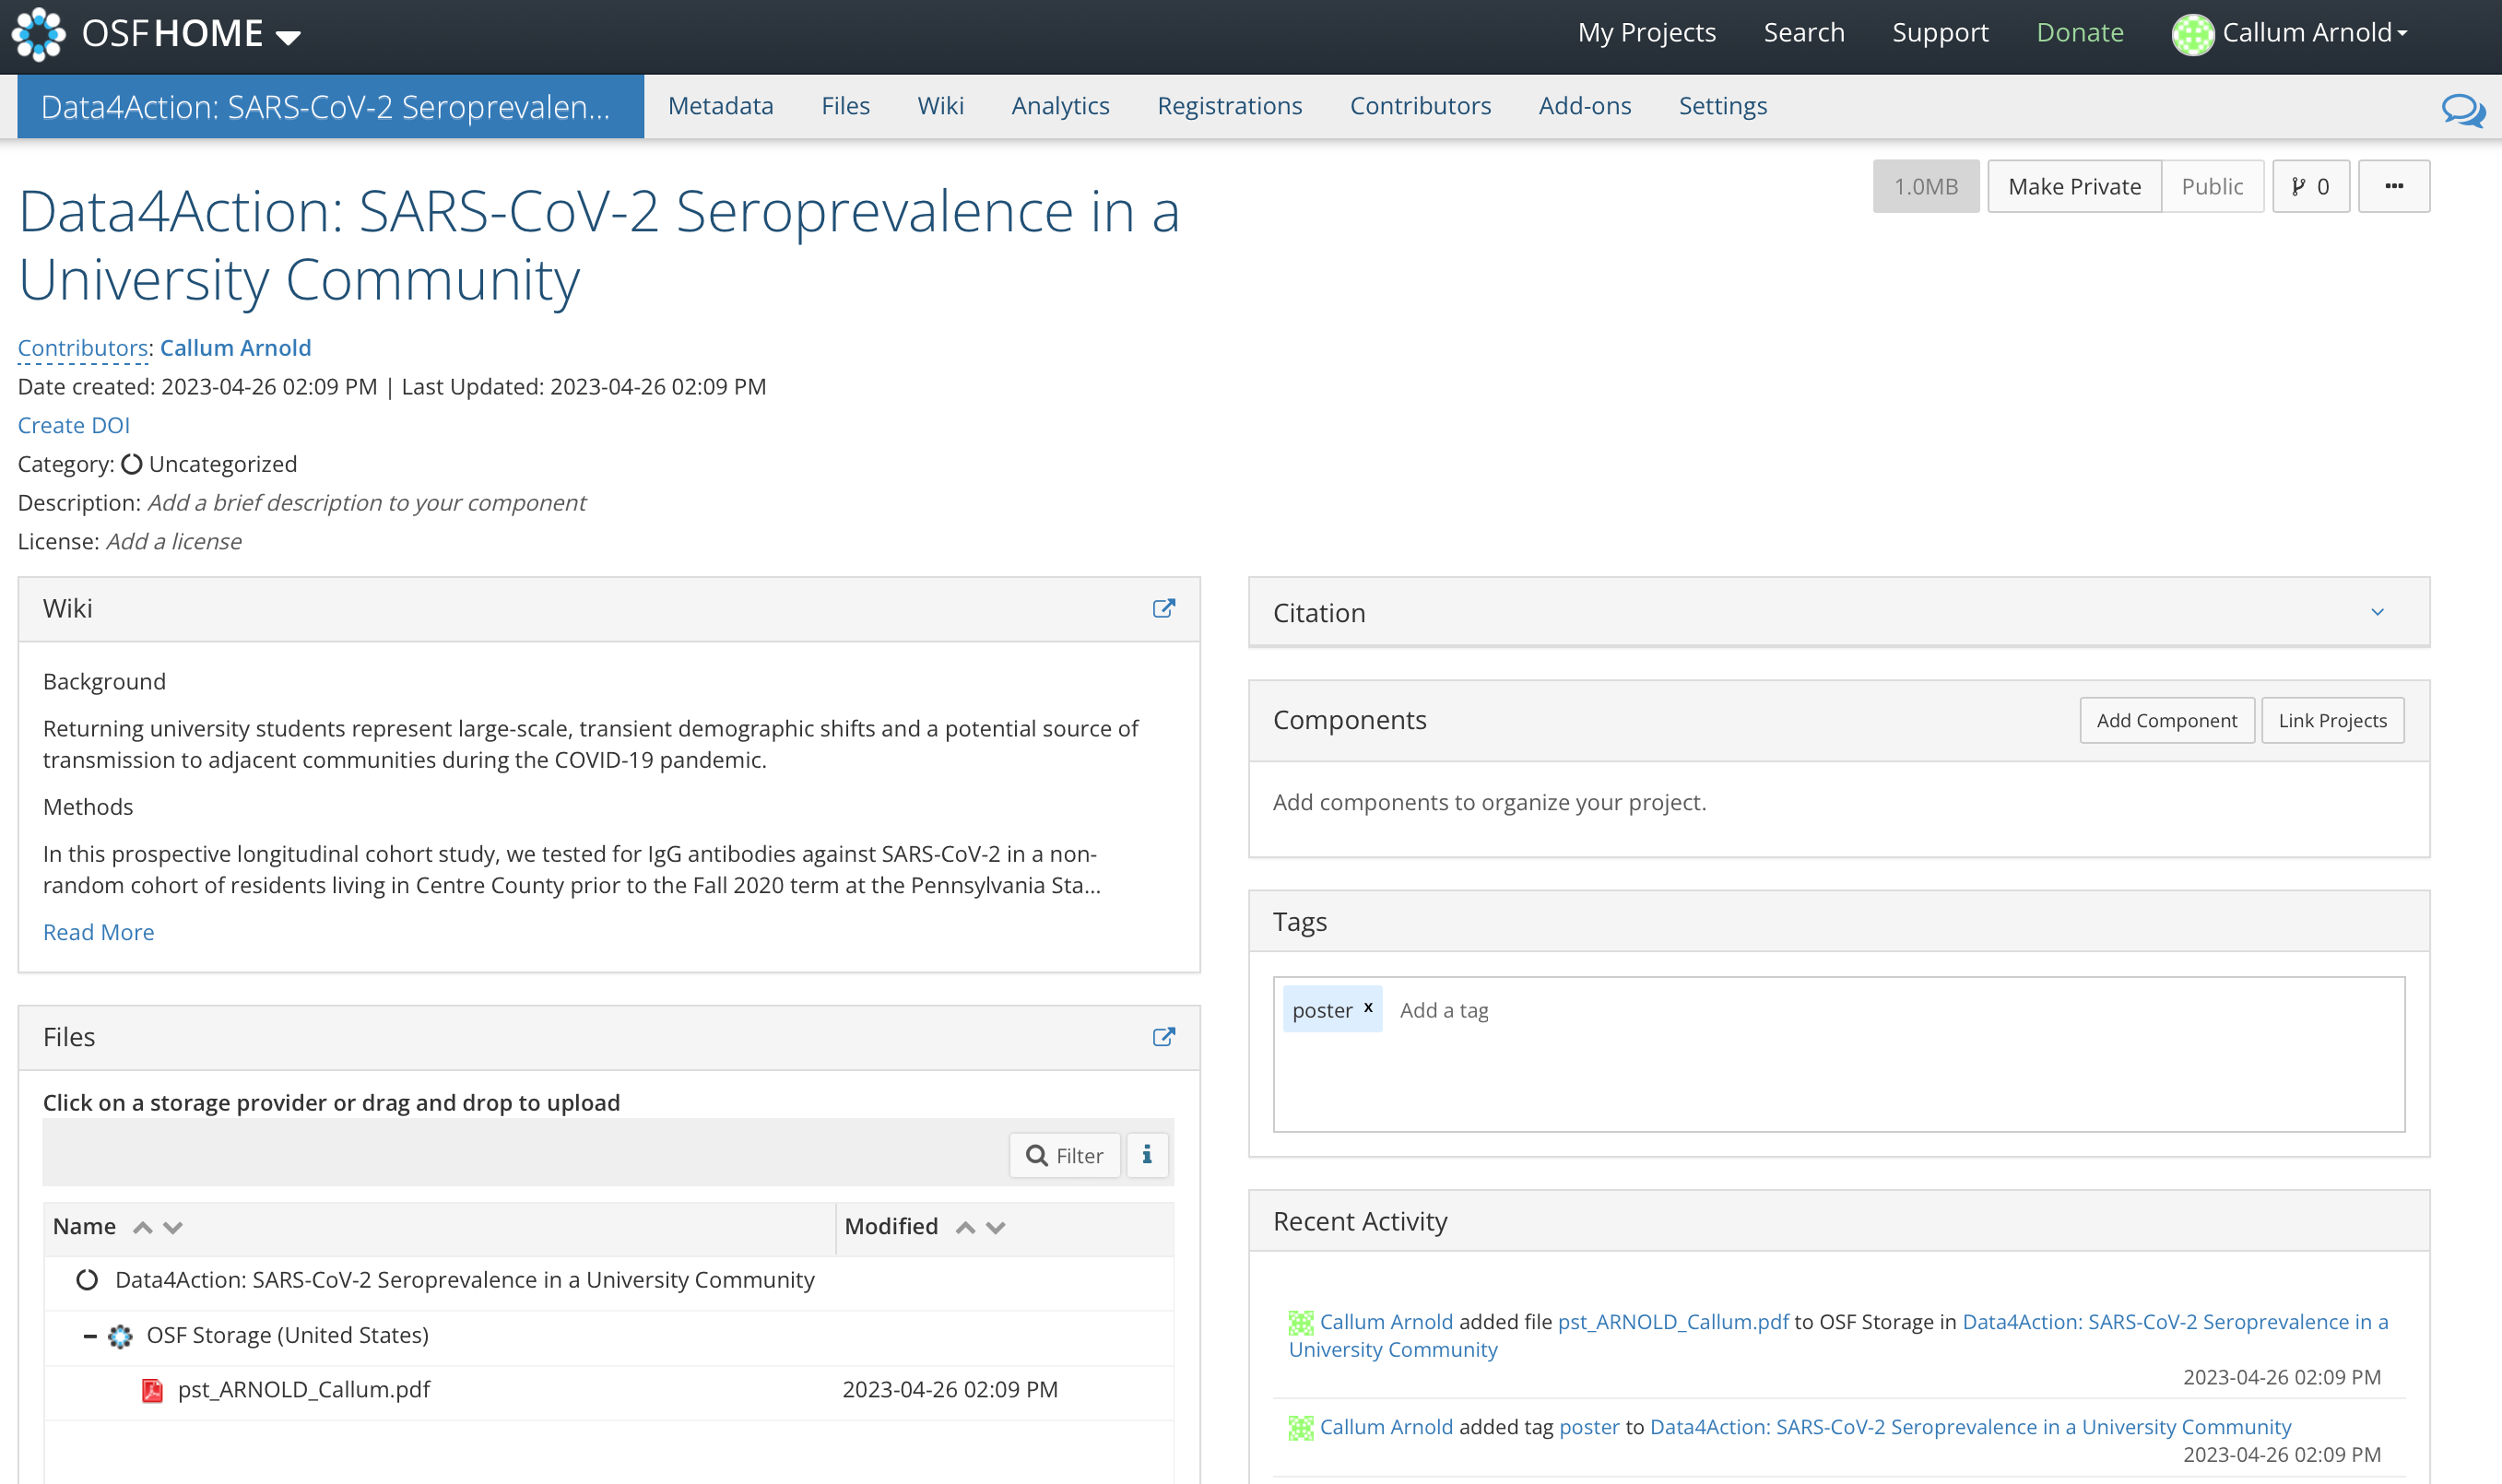
\includegraphics[width=\textwidth]{project-page-01.png}
    \caption{OSF Project Page}
\end{figure}

The main things to note on this page are:

\begin{itemize}
    \item \textbf{Title}: This is the title of your poster/talk, and is exactly what you put in the subject line of your email.
    \item \textbf{Wiki}: This is where your abstract will be displayed.
    Clicking on the up-arrow button in the top-right corner of the Wiki box will allow you to edit the abstract, including adding formatting to delineate sections.
    \item \textbf{Create DOI}: Under the title, there is an option to create a DOI for your poster/talk, that is permanently linked to this project page.
    \item \textbf{Citation}: Automatically generated citations for your project.
    \item \textbf{Files}: This shows what files are attached to your project, and where they are stored.
    At a minimum, this section should contain your poster or talk file, but please feel free to add additional files that you think would provide useful context.
    These files could include slides or videos describing your work, related manuscripts or preprints related, the data files and code used to generate your presentation, etc.
    By default, your poster file is stored on OSF directly, but you can link other storage services (e.g., Google Drive, Dropbox, etc.) to your OSF account and project, and upload other files to these services that will then be shown here.
    For more information on linking storage services, see \hyperref[sec:linking-services]{this section below.}
    \item \textbf{Recent Activity}: This shows a log of all changes made to the project, including uploading files, editing the Wiki, etc.
\end{itemize}

Your poster/talk will also be added to the EEID 2023 conference page/project, which can be accessed at \href{https://osf.io/meetings/EEID2023}{\texttt{https://osf.io/meetings/EEID2023}}

\section{\underline{Editing Your Poster/Talk}}

\subsection{Accessing Your Poster/Talk Project}

Once you have submitted your poster/talk, you can edit it at any time by logging in to your OSF account, and going to the project page, accessed by clicking on the \emph{My Projects} button in the website toolbar, by directly searching for \href{https://osf.io/myprojects/}{\texttt{https://osf.io/myprojects/}}, or by accessing the project link sent to you in the OSF confirmation of submission email.
Once here, you may need to click on \emph{All my projects and components} button in the left sidebar to show your projects, before navigating to your poster/talk project.

\subsection{Editing the Title}

If you submitted your presentation with a placeholder title in the email \emph{Subject} (or if you would just like to change it), you can do this by going to the \emph{Settings} button in the project toolbar, and clicking on \emph{Change title}. See Figure \ref{fig:title-edit}.

\begin{figure}[!htb]
    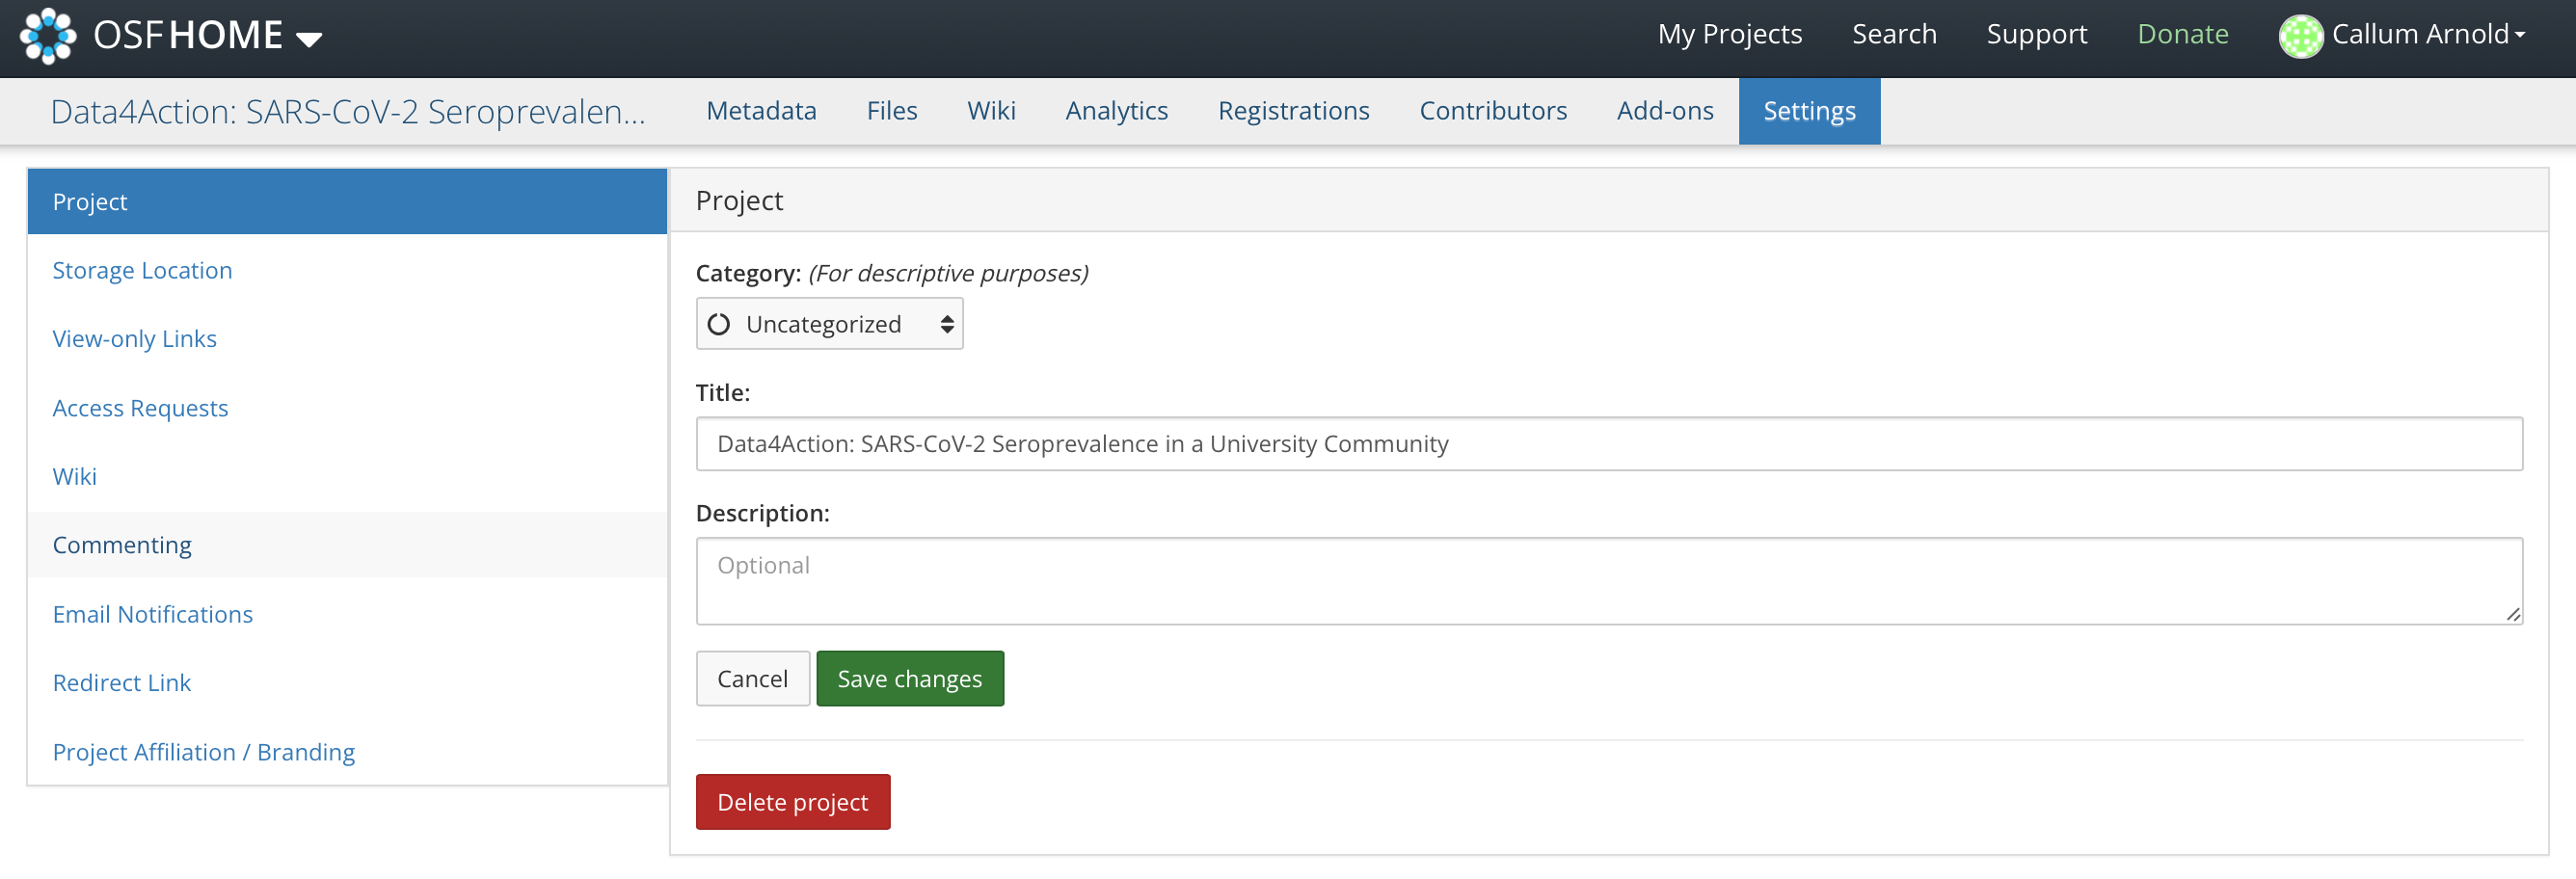
\includegraphics[width=\textwidth]{title-edit.png}
    \caption{Changing the Title}
    \label{fig:title-edit}
\end{figure}

\subsection{Editing the Wiki (Abstract)}

Clicking on the \emph{Wiki} button in the project toolbar will allow you to edit the abstract, using \href{https://www.markdownguide.org/basic-syntax/}{markdown formatting}, as shown in Figure \ref{fig:wiki-edit}.

\begin{displayquote}
    \textbf{Note:} There are three toggle buttons in the top right corner (\emph{View}, \emph{Edit}, and \emph{Compare}) that allow you to preview the changes made, make edits, and compare what has changed related to a previous version, respectively.
\end{displayquote}

\begin{figure}[!htb]
    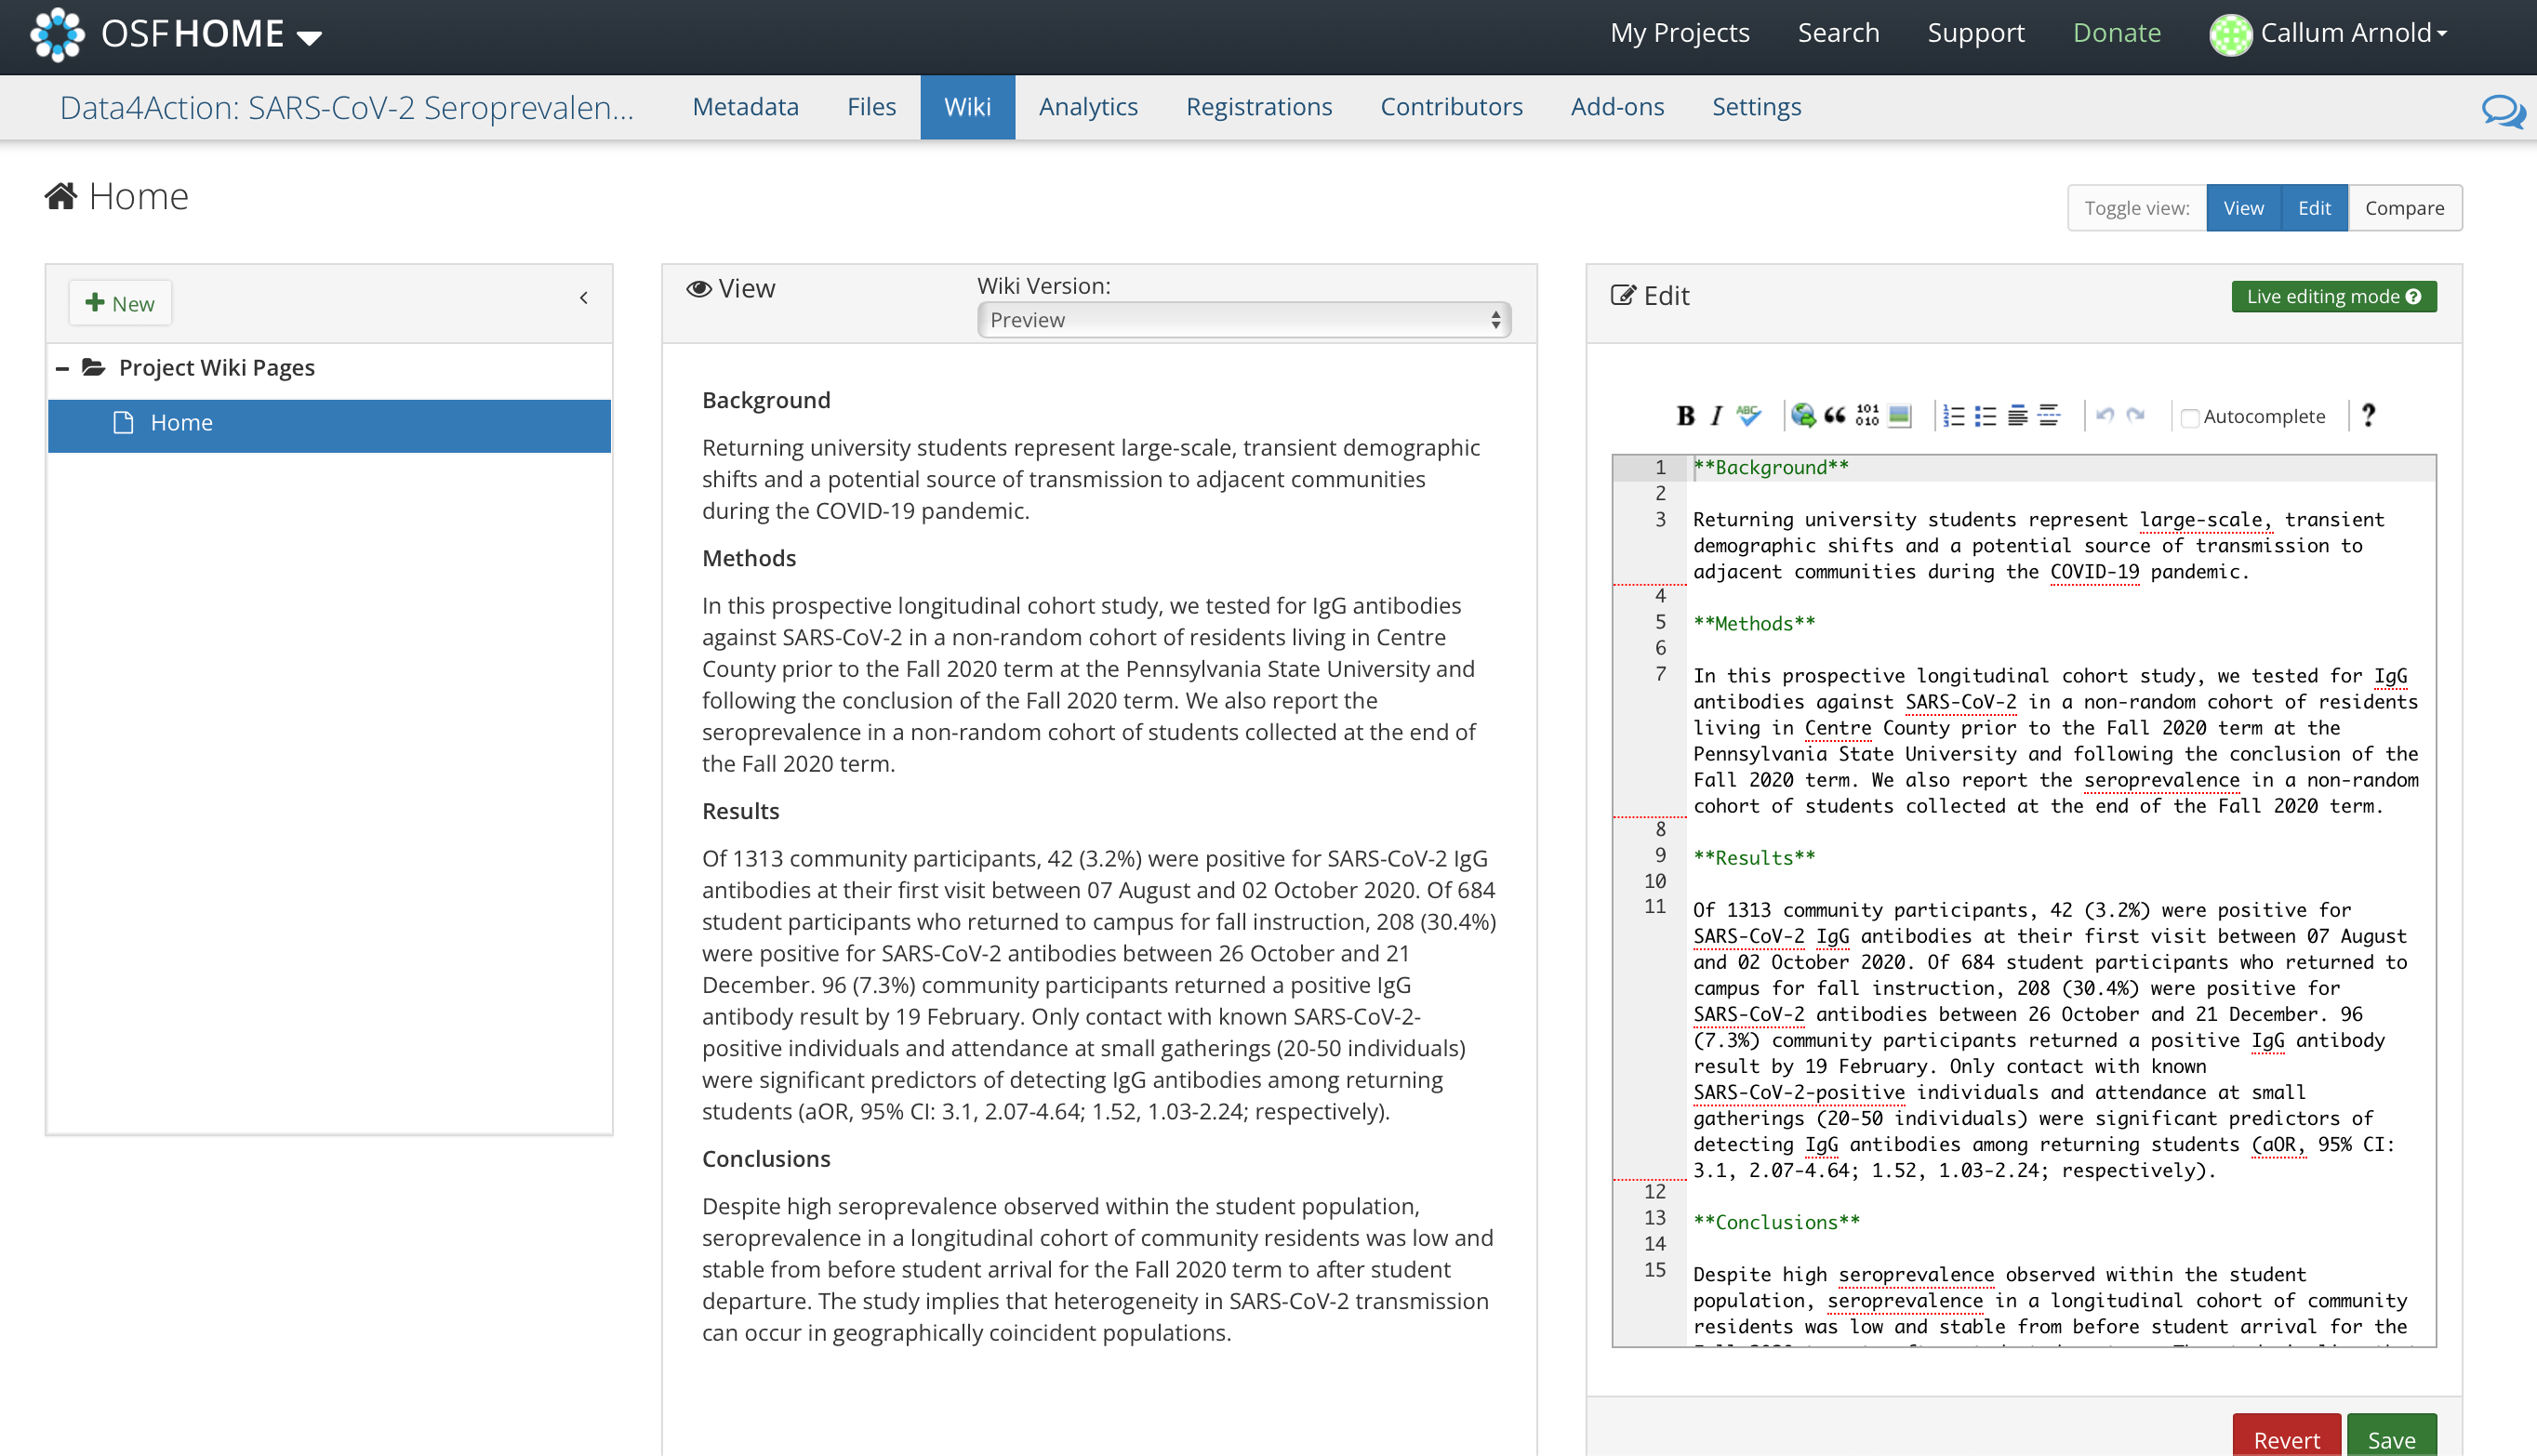
\includegraphics[width=\textwidth]{wiki-edit.png}
    \caption{Editing the Wiki}
    \label{fig:wiki-edit}
\end{figure}

\subsection{Adding/Deleting Files}

Clicking on the \emph{Files} button in the project toolbar will allow you to add/delete files, as well as viewing the files that have been uploaded to the project.
Clicking on the file name will open a preview of the file.
Clicking on the three vertical dots to the right of a file name will allow you to delete, share, download, rename, or move the file.
Clicking on the green plus button in the top-right corner of the Files box will allow you to upload new files to the project.
See Figure \ref{fig:file-edit}.

\begin{figure}[!htb]
    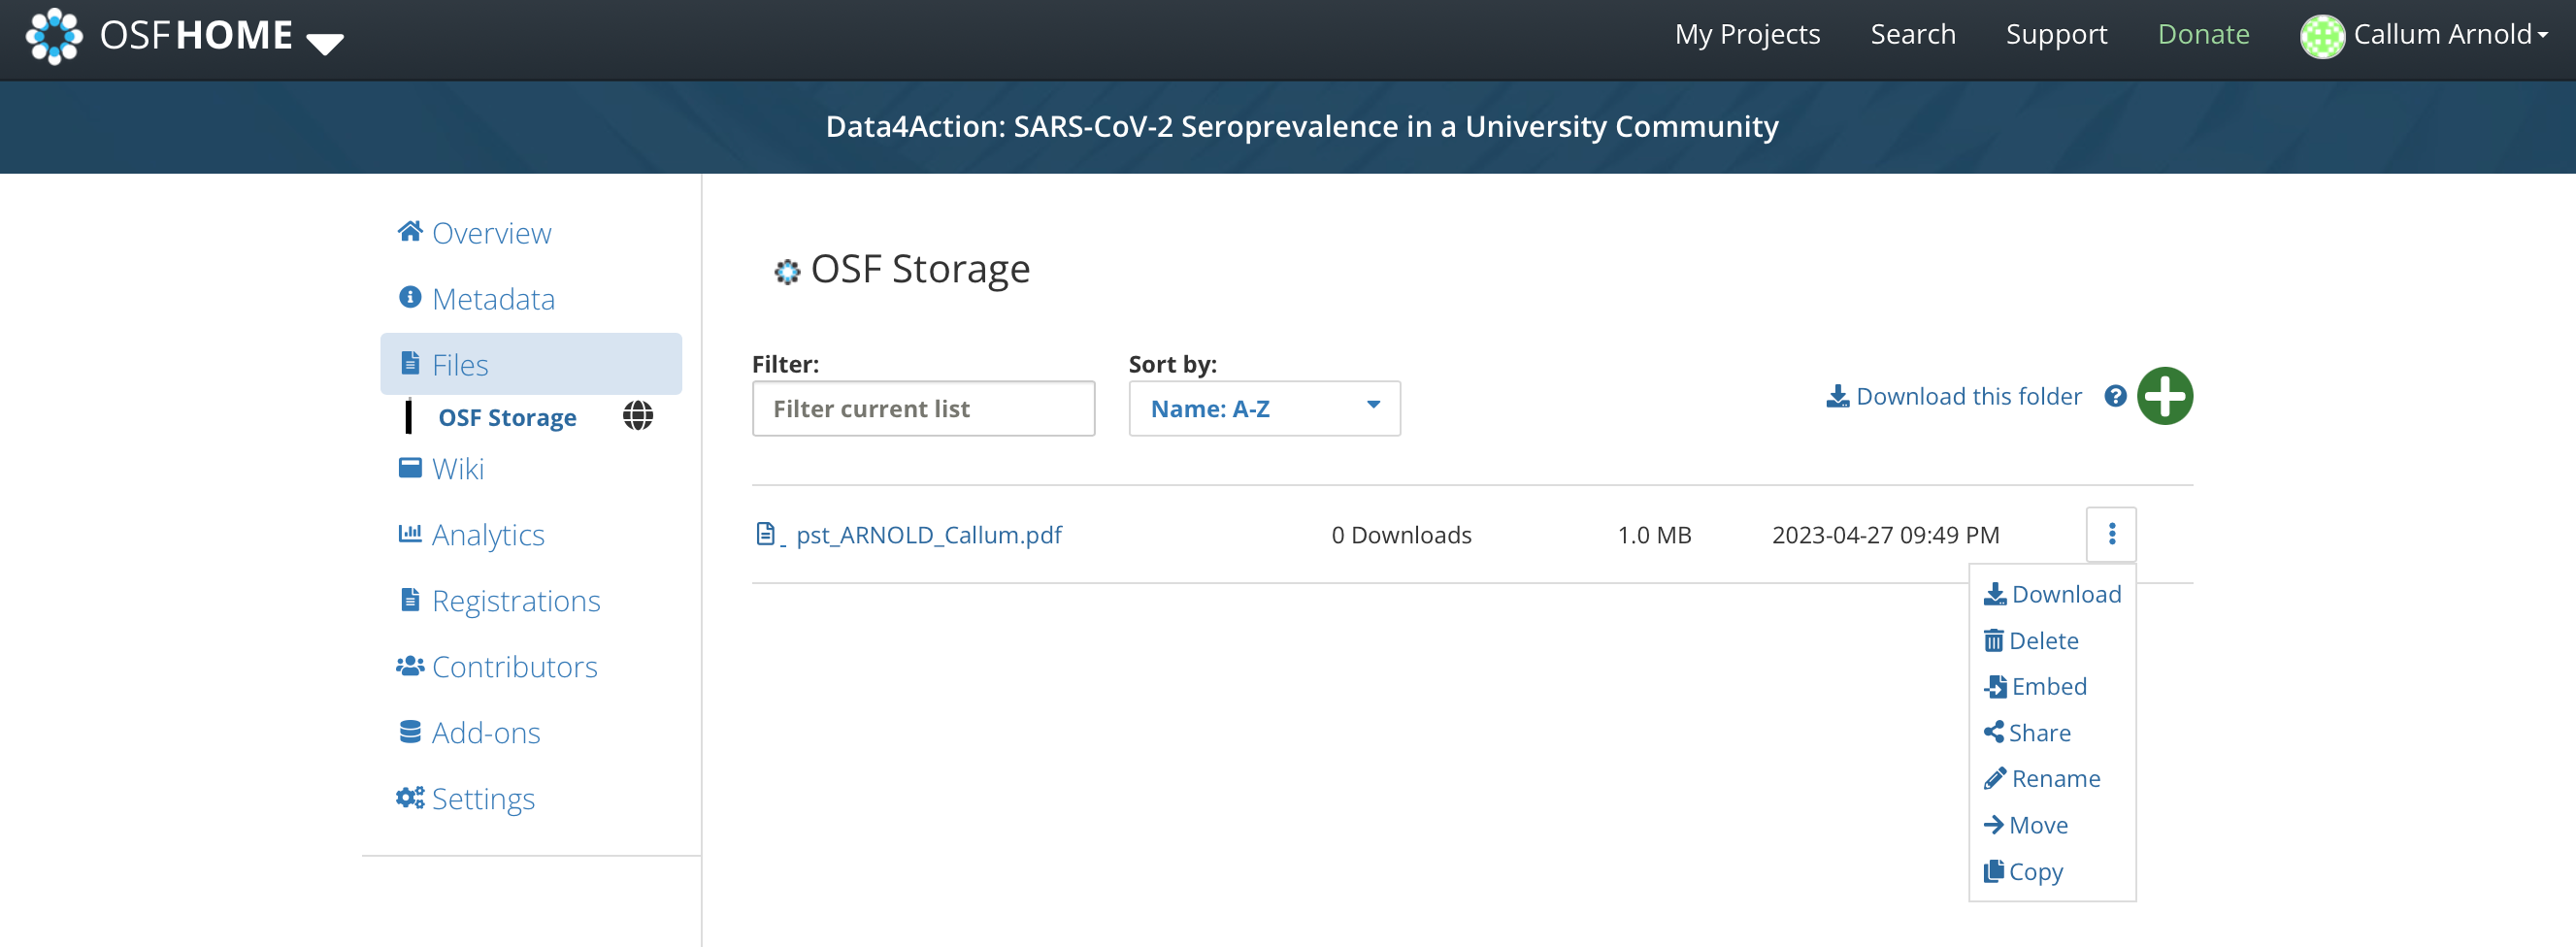
\includegraphics[width=\textwidth]{file-edit.png}
    \caption{Editing Files}
    \label{fig:file-edit}
\end{figure}

\subsection{Linking Other Services}
\label{sec:linking-services}

If you have files stored on other services that you would like to include in your poster/talk project, so they can be easily accessed by attendees, you can do this fairly easily.
Clicking on the \emph{Add-ons} button in the project toolbar allows you to link other services, like GitHub, Dropbox, Google Drive, OneDrive, etc., to your project, and upload files from these services to your project.
However, this is a two-step process.

1) First, you need to link the service to your OSF account.
To do this, first go to your account settings by clicking on your profile picture in the top-right corner of the website, and selecting \emph{Settings}, shown in Figure \ref{fig:addons-account-settings-01}.

\begin{figure}[!htb]
    \centering
    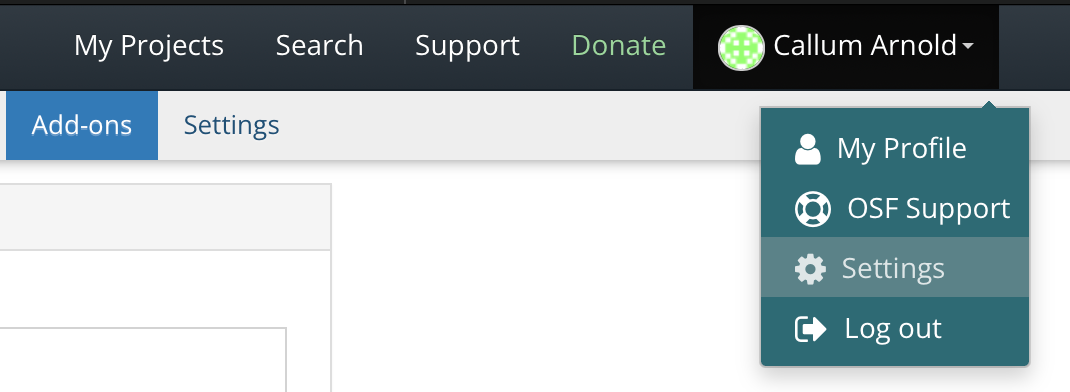
\includegraphics[scale=0.5]{addons-account-settings-01.png}
    \caption{Navigate to Account Settings}
    \label{fig:addons-account-settings-01}
\end{figure}

Then, click on the \emph{Configure add-on accounts} button in the left sidebar, and select the service you want to link, as shown in Figure \ref{fig:addons-account-settings-02}.

\begin{figure}[!htb]
    \centering
    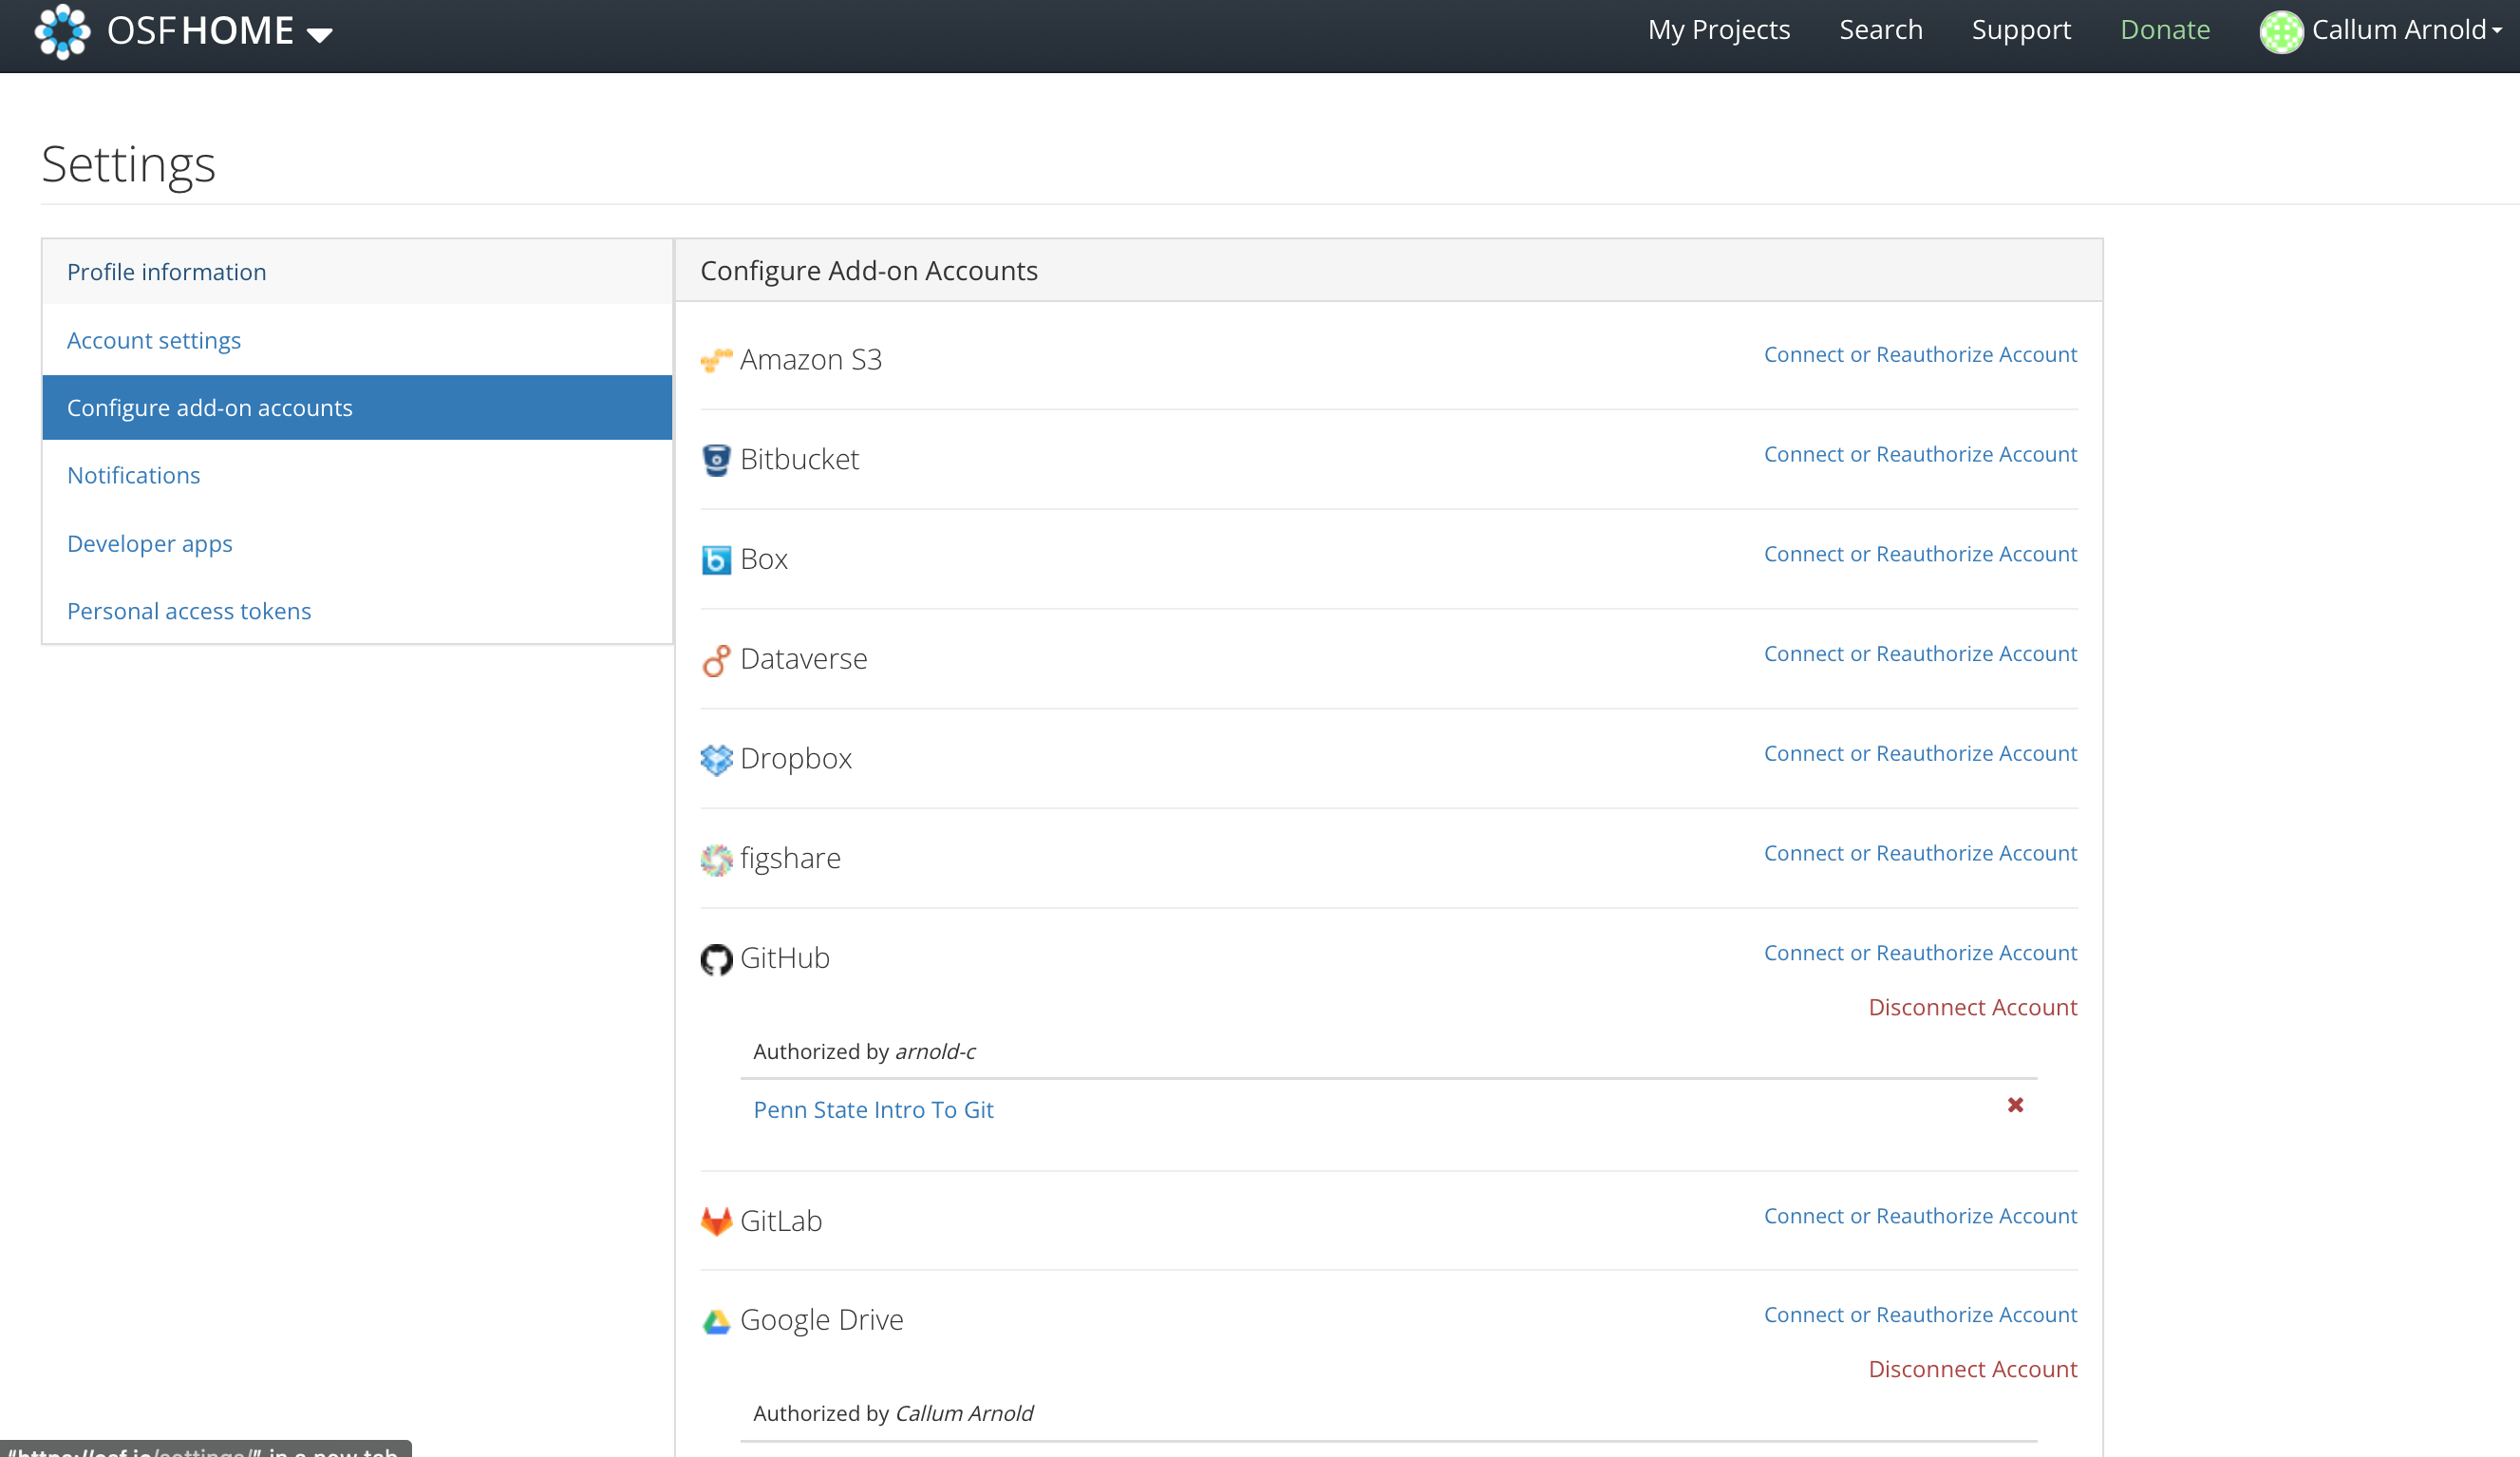
\includegraphics[width=\textwidth]{addons-account-settings-02.png}
    \caption{Connect Your Add-On Account}
    \label{fig:addons-account-settings-02}
\end{figure}

2) Now your OSF account is linked to the service, you can link your project to the service, and specify which files you want to upload to your project.
To do this, go back to your project page, and click on the \emph{Add-ons} button in the project toolbar, and select the service you want to link, as shown in Figure \ref{fig:addons-project-01}.

\begin{figure}[!htb]
    \centering
    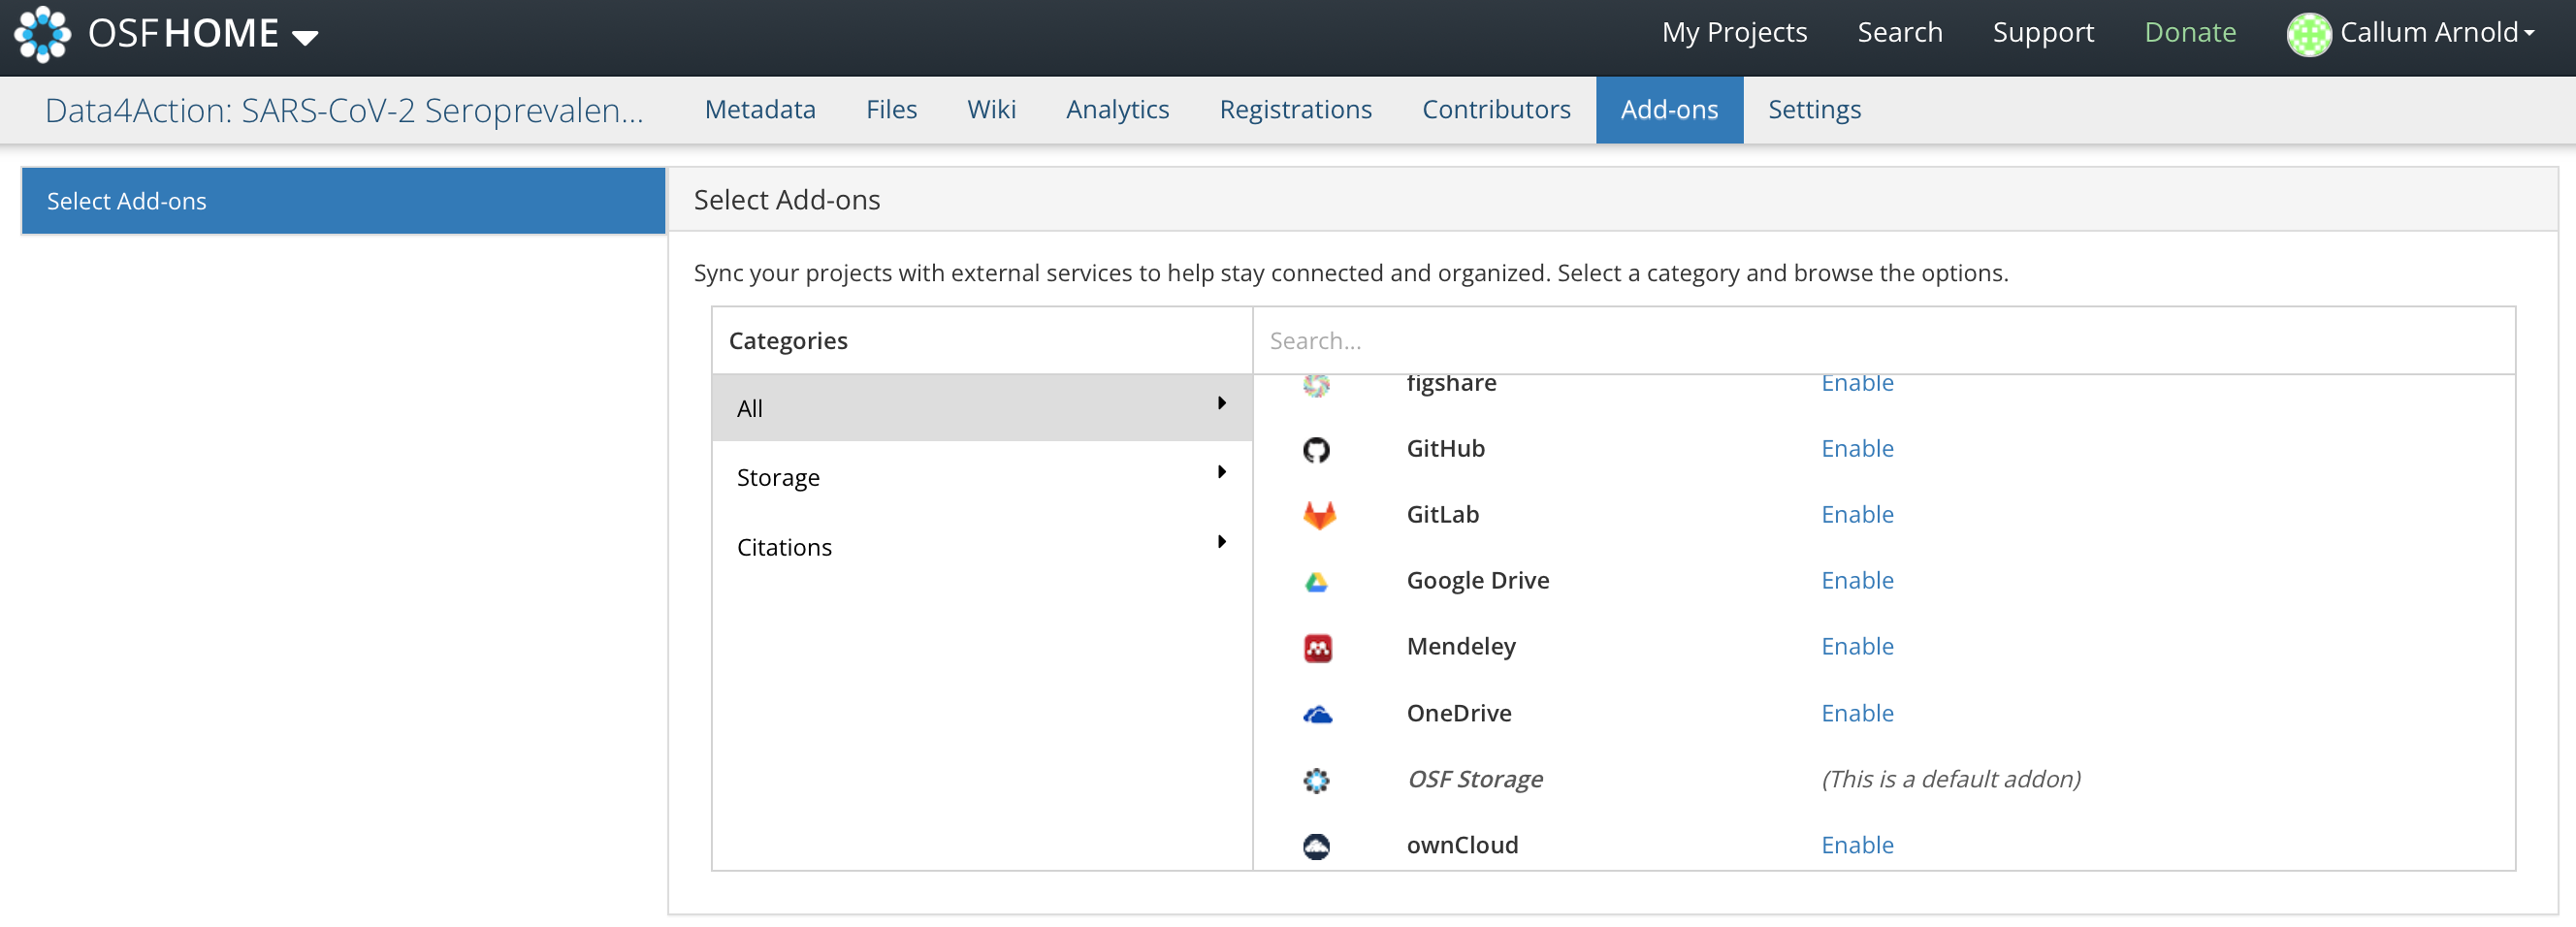
\includegraphics[width=\textwidth]{addons-project-01.png}
    \caption{Connect Your Add-On to Your Project}
    \label{fig:addons-project-01}
\end{figure}

Then, click on the \emph{Import Account from Profile} button, to start the import process, as shown in Figure \ref{fig:addons-project-02}, and select the appropriate files/folders to be imported.

\begin{figure}[!htb]
    \centering
    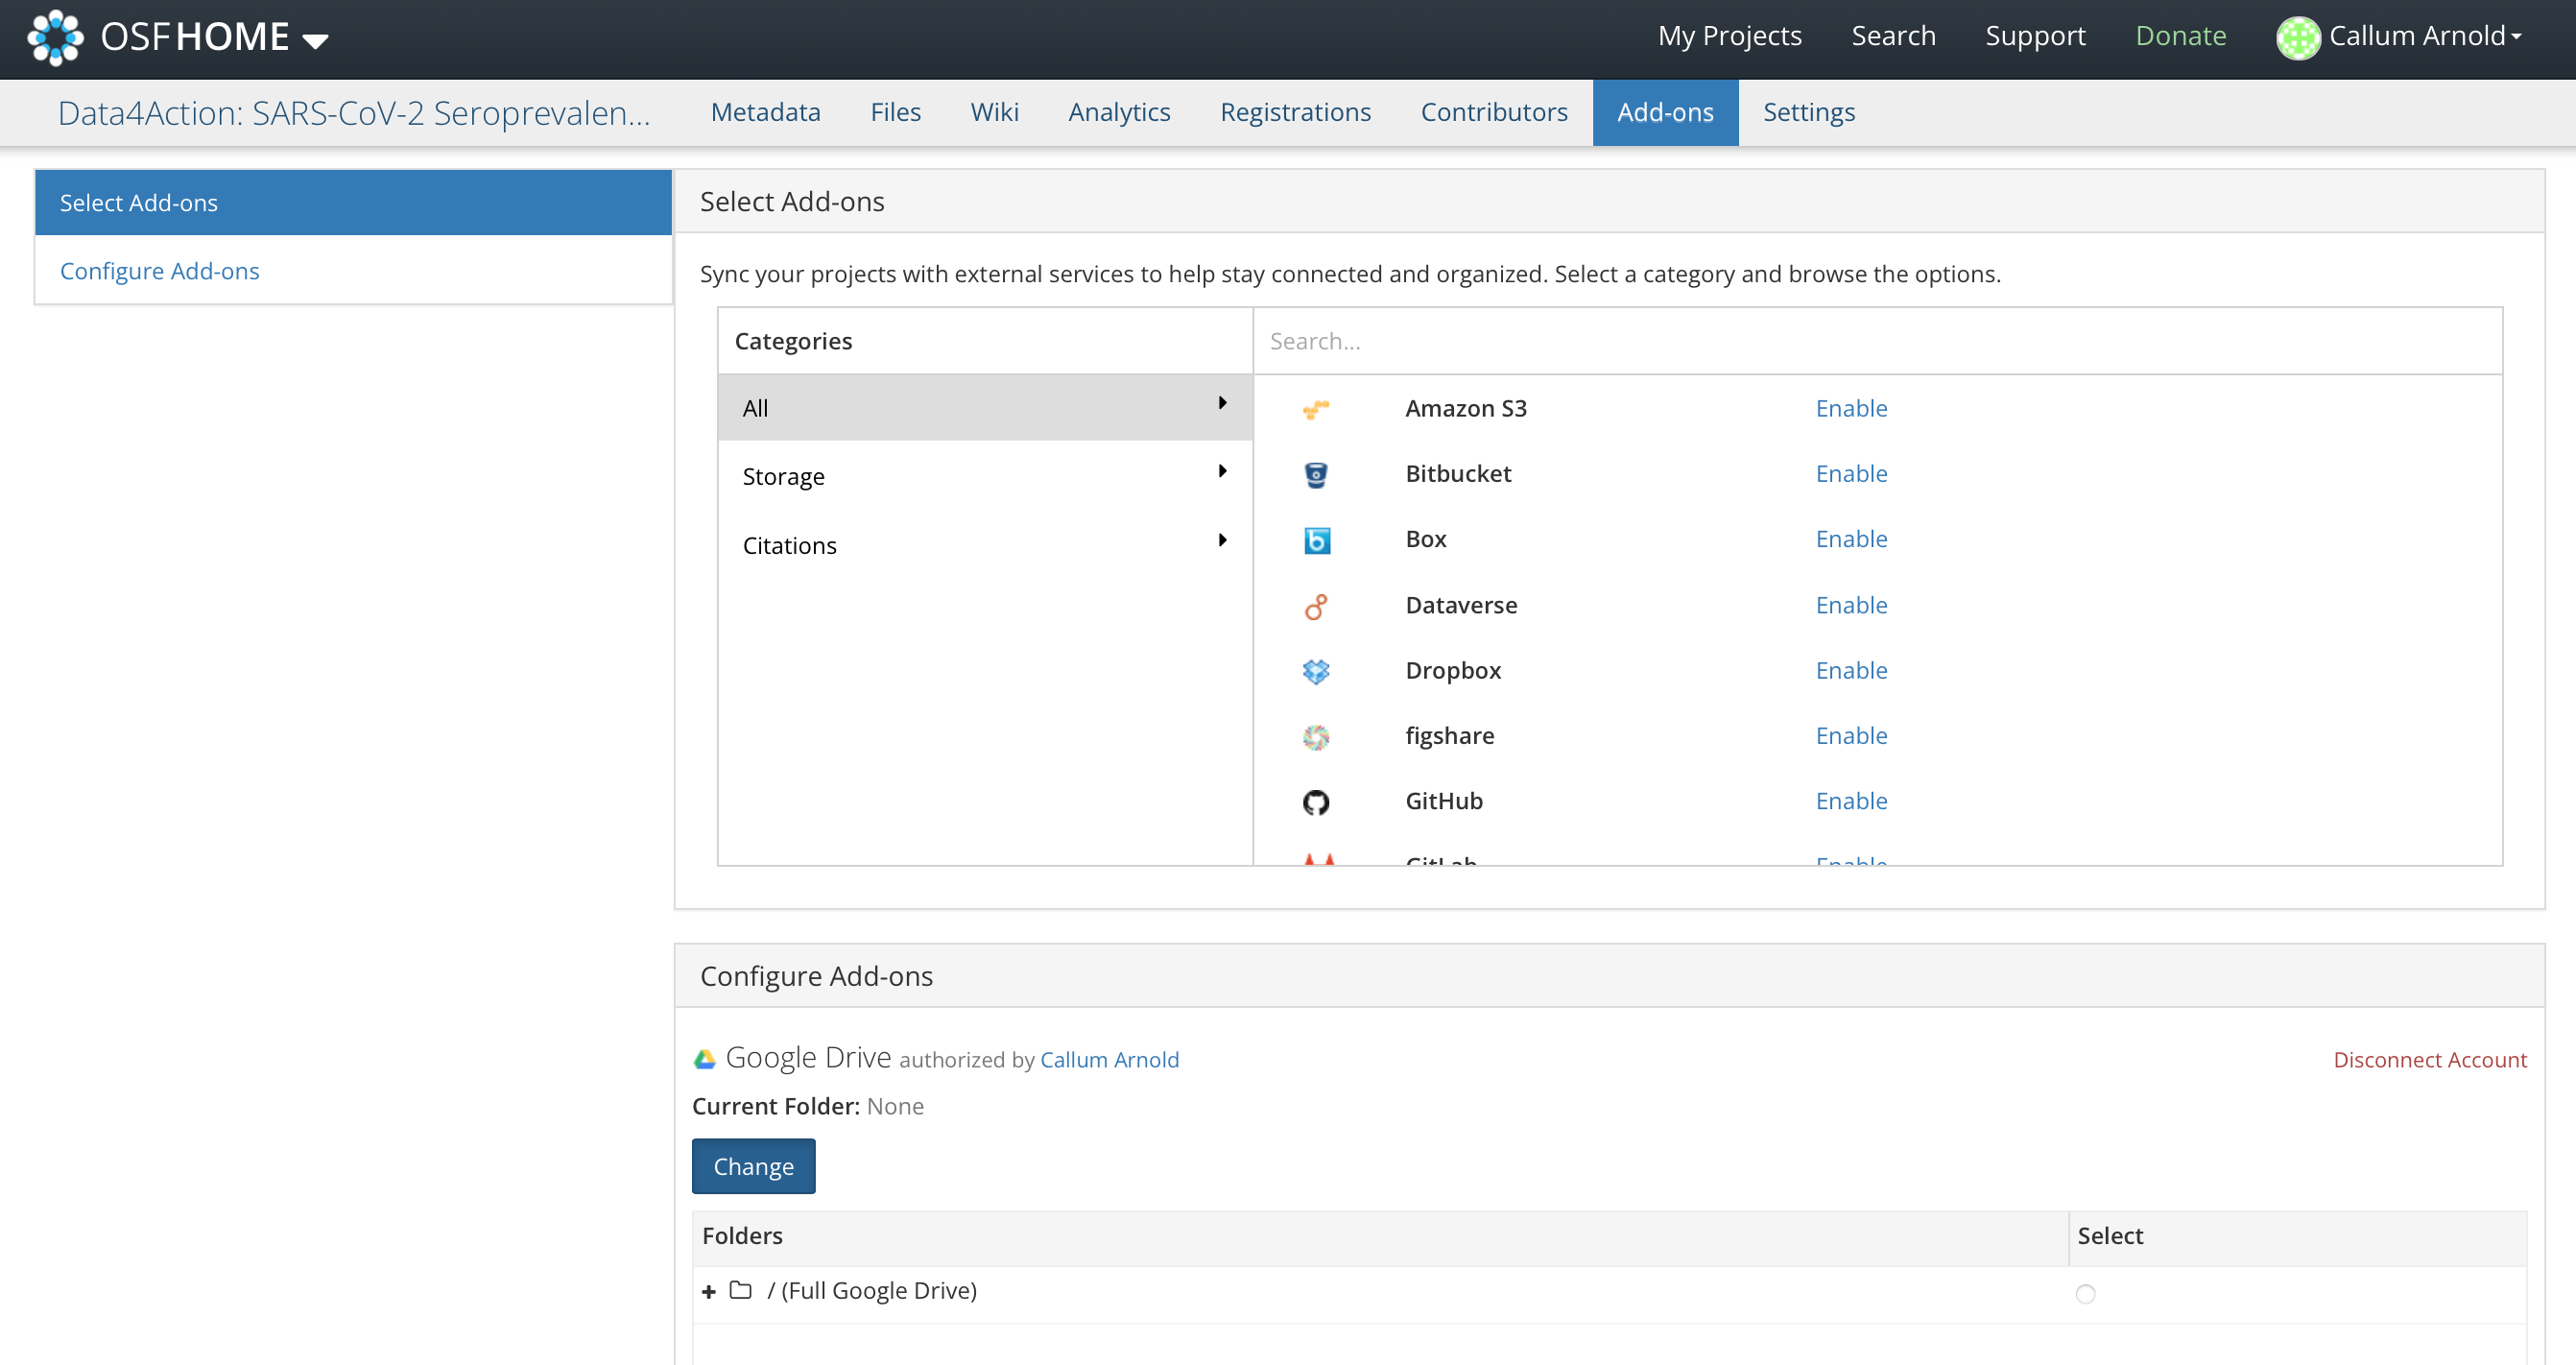
\includegraphics[width=\textwidth]{addons-project-02.png}
    \caption{Import the Project-Specific Files}
    \label{fig:addons-project-02}
\end{figure}

\section{\underline{Troubleshooting Tips}}

The first place to start is the OSF support page, which can be accessed at \href{https://help.osf.io}{\texttt{https://help.osf.io}}.
The five sections that will likely be most useful are:

\begin{enumerate}
    \item \emph{Getting Started}
    \item \emph{Account and Security}
    \item \emph{Projects and Components}
    \item \emph{Add-ons \& API Integrations}
    \item \emph{FAQs}
\end{enumerate}

\subsection{Unable to Log In}

If for some reason you are unable to log in to your OSF account shortly after setting up your account, and you are unable to reset the password, there may have been an issue with how your email address was associated with your account.
This seems to be more of an issue with email addresses that have been transferred from ORCiD during account creation i.e. \emph{Sign up with ORCiD}.

One potential fix is to set up a brand new account with a different email address, and then merge the old account into the new one (assuming you know the email address associated with the old account).
To do this, log in to the new account, and go to the \emph{Settings} page, by clicking on your profile picture in the top-right corner of the website, and selecting \emph{Settings}.
Then, click on the \emph{Account settings} button in the left sidebar, and enter the email address associated with the old account into the box under \emph{Unconfirmed emails} before clicking \emph{Add email}, as shown in Figure \ref{fig:merge-accounts}.

\begin{figure}[!htb]
    \centering
    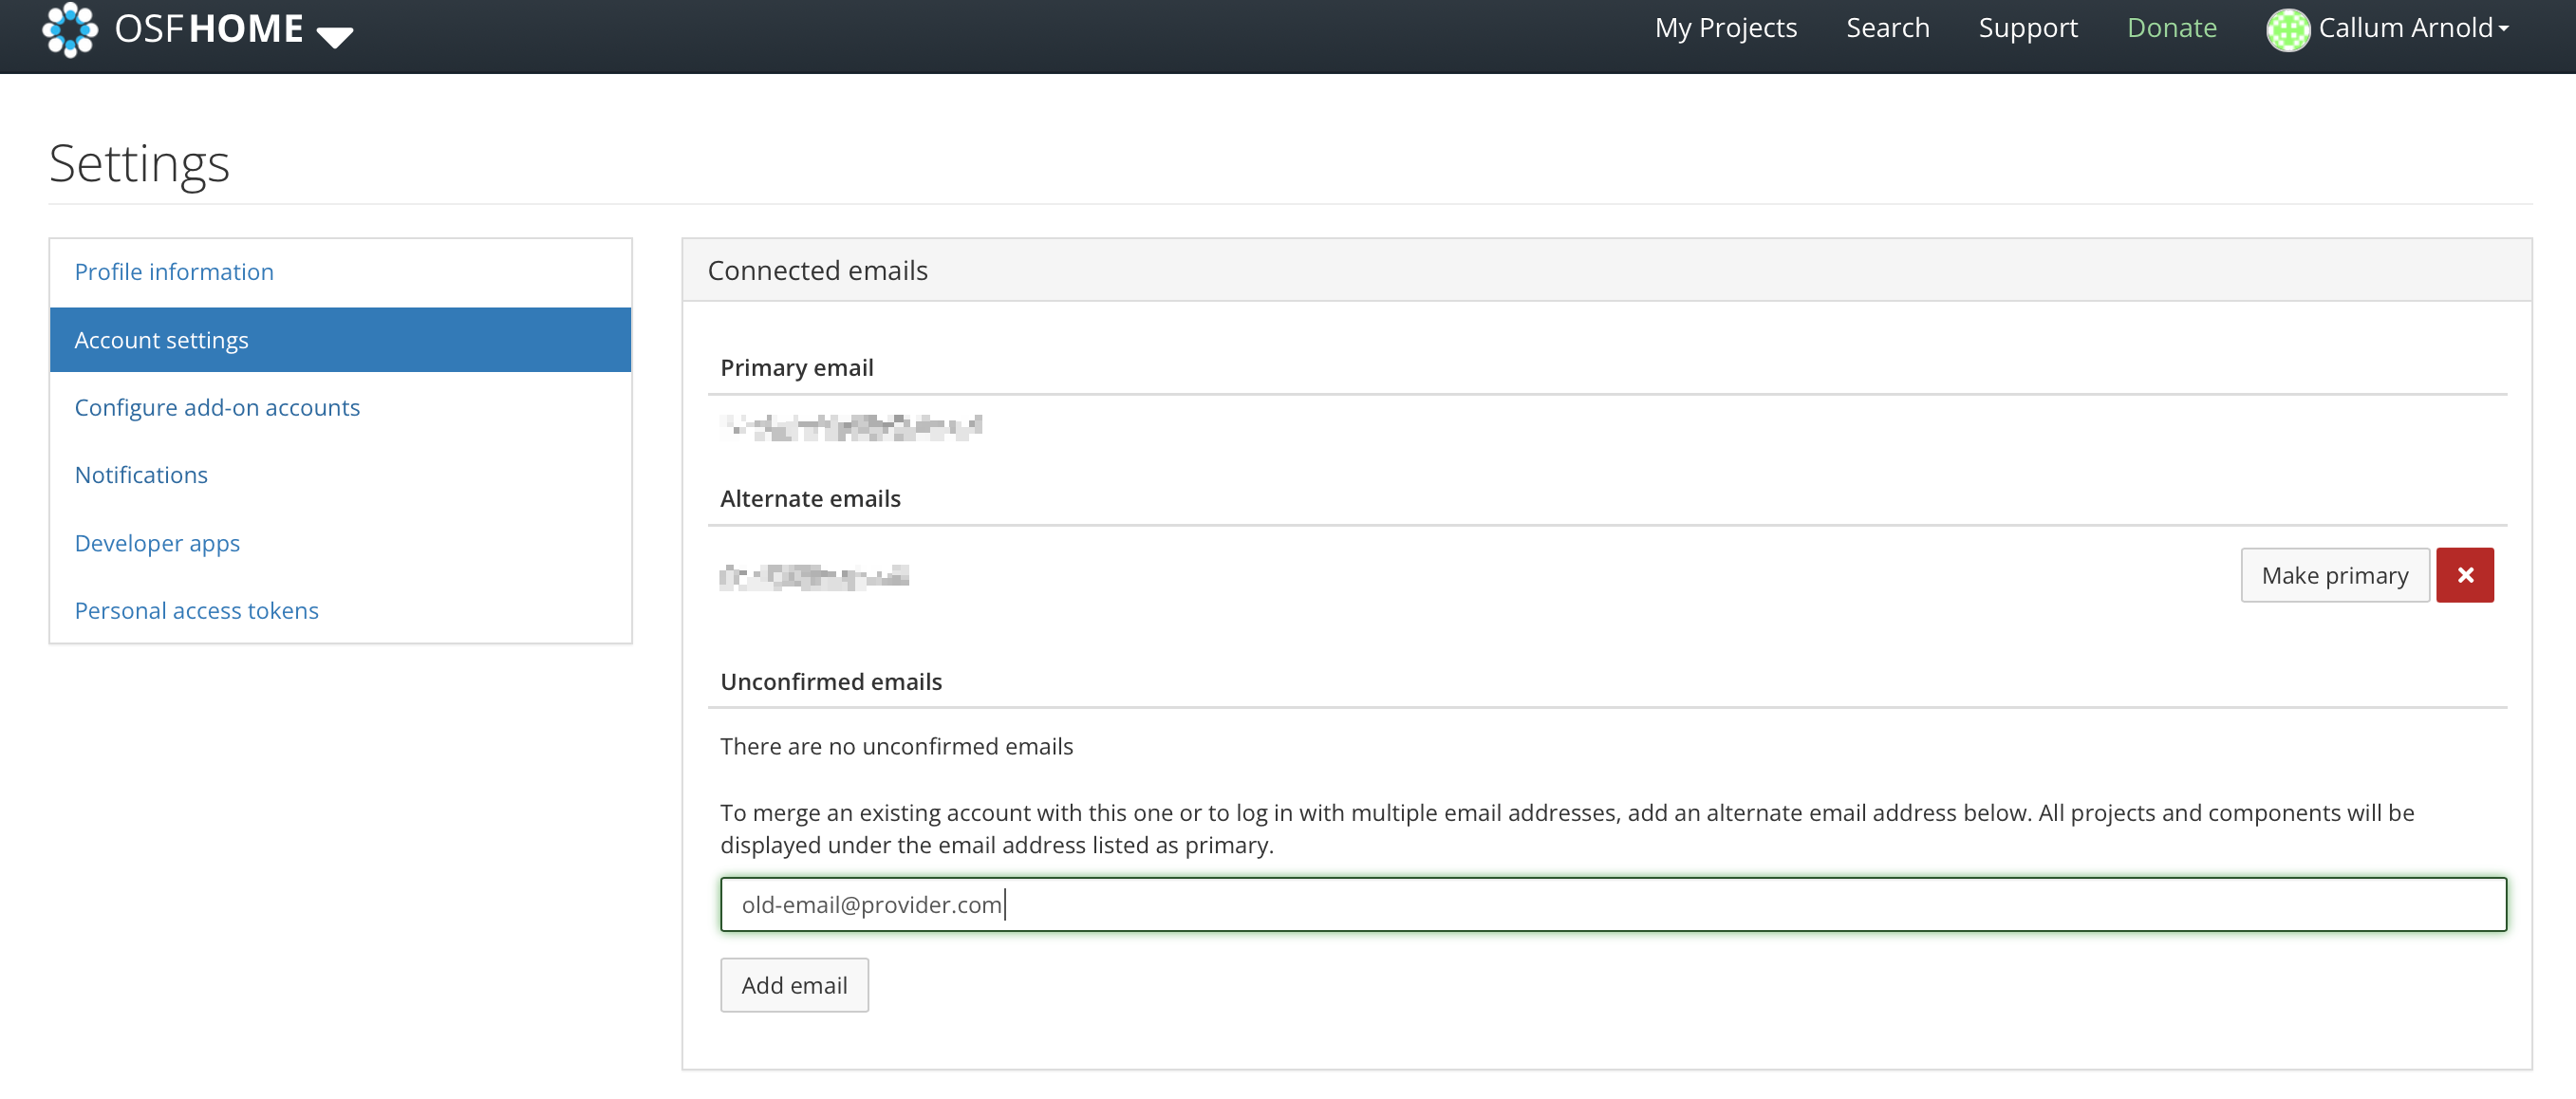
\includegraphics[width=\textwidth]{merge-accounts.png}
    \caption{Merge Accounts}
    \label{fig:merge-accounts}
\end{figure}

\end{document}